\subchapter
{Root filesystem construction}
{Objectives:}

\section{Explore the build output}

\section{Configure the network on your host}

In the next sections of this lab, we will want to interact with the
BeagleBone Black over the network. So in this section, we'll configure
an Ethernet interface on your host machine.

With a network cable, connect the Ethernet port of your board to the
one of your computer. If the main wired Ethernet port of your computer
is already used, your instructor will provide you with a USB Ethernet
adapter. A new network interface, probably \code{eth1} or \code{eth2},
should appear on your Linux system.

To configure this network interface on the workstation side, click on
the {\em Network Manager} tasklet on your desktop, and select {\em
Edit Connections}.

\begin{center}
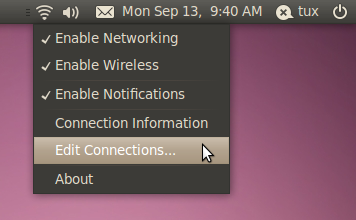
\includegraphics[width=8cm]{labs/buildroot-rootfs/network-config-1.png}
\end{center}

Select the new {\em wired network connection}:

\begin{center}
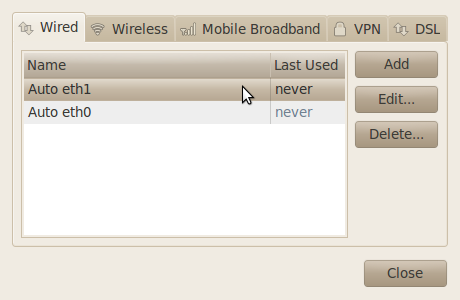
\includegraphics[width=8cm]{labs/buildroot-rootfs/network-config-2.png}
\end{center}

In the \code{IPv4 Settings} tab, press the \code{Add} button
and make the interface use a static IP
address, like \code{192.168.0.1} (of course, make sure that this
address belongs to a separate network segment from the one of the main
company network).

\begin{center}
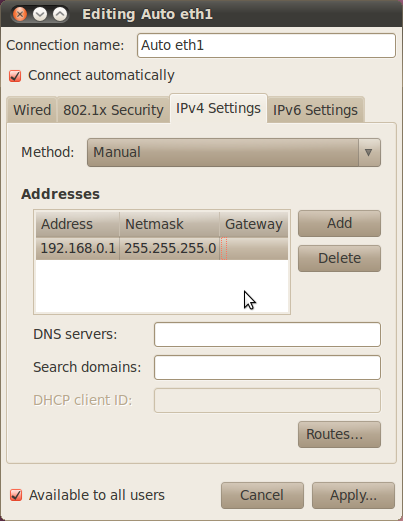
\includegraphics[width=8cm]{labs/buildroot-rootfs/network-config-3.png}
\end{center}

You can use \code{255.255.255.0} as \code{Netmask}, and leave the
\code{Gateway} field untouched (if you click on the \code{Gateway} box, you
will have to type a valid IP address, otherwise you won't be apply to
click on the \code{Apply} button).

{\em Note: using \code{ifconfig} in the command line is not
recommended, because Network Manager will unconfigure and reconfigure
the network interface each time the cable is unplugged or each time
the board reboots.}

\section{Add {\em dropbear} as an SSH server}

As a first additional package to add to our system, let's add the {\em
dropbear} SSH client/server. The server will be running on the
BeagleBone Black, which will allow us to connect over the network to
the BeagleBone Black.

Run \code{make menuconfig}, and enable the \code{dropbear}
package. You can use the search capability of \code{menuconfig} by
typing \code{/}, enter \code{DROPBEAR}. It will give you a list of
results, and each result is associated with a number between
parenthesis, like \code{(1)}. Then simply press \code{1}, and
\code{menuconfig} will jump to the right option.

After leaving \code{menuconfig}, restart the build by running
\code{make}.

In this case, we do not need to do a full rebuild, because a simple
\code{make} will notice that the \code{dropbear} package has not been
built, and will therefore trigger the build process.

Re-extract the root filesystem tarball in the \code{rootfs} partition
of the SD card. Don't forget to replace the entire root filesystem:

\begin{verbatim}
rm -rf /media/<user>/rootfs/*
sudo tar -C /media/<user>/rootfs/ -xf output/images/rootfs.tar
\end{verbatim}

Now, boot the new system on the BeagleBone Black. You should see a
message:

\begin{verbatim}
Starting dropbear sshd: OK
\end{verbatim}

Log in the system, and configure an IP address manually by doing
\code{ifconfig eth0 192.168.0.2}. Now, from your host machine, you can
connect over the network to the board by doing \code{ssh
root@192.168.0.2}.

However, configuring the IP address every time you boot the board is
not very practical, so let's move to the next section, in which we
will learn how to do this properly.

\section{Use a {\em rootfs overlay} to configure the IP address}

By default, Buildroot uses the \code{ifup} program from Busybox, which
reads the \code{/etc/network/interfaces} file to configure network
interfaces.

So, we could write a \code{/etc/network/interfaces} file on our
target, and reboot. However, the next time we will fully rebuild and
reflash our system, such changes will have disappeared. It is
important that our build process remains fully reproducible, so we
want to ensure that the next build will include such custom
configuration.

To achieve this, the easiest way is to use the {\bf rootfs overlay}
mechanism of Buildroot. Since this {\em overlay} is specific to our
project, we will create a custom directory for our project within the
Buildroot sources: \code{board/felabs/beagleboneblack/}.

Within this directory, create a \code{rootfs-overlay} directory, and
in \code{menuconfig}, specify
\code{board/felabs/beagleboneblack/rootfs-overlay} as the {\em rootfs
overlay} (option \code{BR2_ROOTFS_OVERLAY}).

Then, in \code{board/felabs/beagleboneblack/rootfs-overlay}, create a
file named \code{etc/network/interfaces} with the following contents:

\begin{verbatim}
auto lo
iface lo inet loopback

auto eth0
iface eth0 inet static
      address 192.168.0.2
      netmask 255.255.255.0
\end{verbatim}

Then, rebuild your system by running \code{make}. Here as well, we
don't need to do a full rebuild, since the {\em rootfs overlays} are
applied at the end of each build. You can check in
\code{output/target/etc/network/interfaces} if the contents of the
file are good.

Reflash the root filesystem on the SD card, and boot your BeagleBone
Black. It should now have an IP address configured for \code{eth0} by
default.

\section{Linux kernel customization}

\section{Add and use {\em input-tools}}

\section{Generate a {\em defconfig}}

\section{Testing a full rebuild}
